\documentclass[../PhysicsFormulae.tex]{subfiles}
\begin{document}
\subsection{Temperature}
Consider two systems separated by a wall. If the wall does not allow heat transfer between the systems, it is adiabatic, or thermally insulating. But if the wall allows heat transfer, it is diathermic, or thermally conducting. Now consider two systems are in thermal contact, but there is no heat transfer, they are in thermal equilibrium. Thus, we can state a postulate known as the \textbf{zeroth law of thermodynamics}: \bigskip

\textit{If systems A and B are in thermal equilibrium with third system C, then A and B are in thermal equilibrium with each other.} \bigskip

The zeroth law allows us to establish \textit{temperature}: when two systems are in thermal equilibrium, we say that they have the same temperature. In practical physics, system C is referred to as a thermometer. We can restate the zeroth law in terms of temperature: \bigskip

\textit{Temperature is a scalar property of all thermodynamic systems in equilibrium. Two systems are in thermal equilibrium iff their temperatures are equal.}
\subsection{Temperature Scales}
There are three scales: Kelvin, Celsius (formerly centigrade), and Fahrenheit. The Kelvin scale is defined as follows: 
\begin{itemize}
\item 0 K is absolute zero, and 273.16 K is the triple point of water. 
\item $0^{\circ}$ C is the freezing point of water; $100^{\circ}$ its boiling point. However, this definition has been swapped for one based on a conversion from the Kelvin scale, changing them to $0.00^{\circ}$ C and $99.975^{\circ}$. 
\item $32^{\circ}$ F is the freezing point of water; $212^{\circ}$ F its boiling point. Again, this definition is historical only. 
\end{itemize}
The relations between the scales are as follows: 
\[ T_F = \left(\frac{9 \; \textrm{F}^{\circ}}{5 \; \textrm{C}^{\circ}}\right) T_C + 32^{\circ} \textrm{F} \]
\[ T_C = \left(\frac{1 \; \textrm{C}^{\circ}}{1 \; \textrm{K}}\right) T_K - 273.15^{\circ} \textrm{C} \]
and the relation between Fahrenheit and Kelvin can be found from substitution. Thus, $9 \; \textrm{F}^{\circ} = 5 \; \textrm{C}^{\circ}$. Notice how the degree symbol comes after the scale symbol when describing temperature intervals.

\subsection{Thermometers}
In principle, any object with a property that varies with temperature can be used as a thermometer. These properties may include gas pressure, resistance of a wire, length of a metal strip, color of a lamp filament, and more. However, the rules for these "private thermometers" is as follows: 
\begin{itemize}
\item \textit{A device-sensative temperature scale is defined only for that property; it does not necessarily agree with other private scales. However, all thermometers agree on the triple point of water (by definition)}. 
\end{itemize}
However, these thermometers are still useful as secondary standards for measuring temperature. \bigskip

Let's analyze thermometers based on properties that vary linearly with temperature; that is, 
\[ T^{*}(X) = (273.16\;\textrm{K}) \frac{X}{X_{tr}} \]
where $T^{*}$ is the private temperature and $X$ is the property used to measure it. This relation must hold because at at triple point, the temperature must be 273.16 K no matter the scale. \bigskip

The Constant-Volume Gas Thermometer is officially used for measuring temperatures because it is independent of the type of material (gas) used. 

\subsection{Thermal Expansion}
Hot things make objects grow larger (as ladies know very well). The linear change in a solid is given by 
\[ \Delta L = \alpha L \Delta T \]
where $\alpha \; [^{\circ}C^{-1}]$ is the coefficient of linear expansion (representing the fractional change in length per unit temperature), on the order of $10^{-5} \sim 10^{-6}$. Strictly speaking, this coefficient does depend on the reference (initial) temperature, but generally these effects are negligible. However, the more accurate equation is 
\[ L \approx L_0 \left[1+\int_{T_0}^{T} \alpha(T)dT\right] \]
For isotropic solids, the percent change in length for a given temperature change is the same for all lines in the solid, meaning that every this change is the same for all diagonals, lengths, widths, etc. Thus, it can also be shown that to a very good approximation, the changes in area and volume are
\[ \Delta A = 2\alpha A \Delta T \]
\[ \Delta V = 3\alpha V \Delta T \]
For liquids, linear expansion is a bit meaningless due to their capability of flowing easily, but volume is still relevant: 
\[ \Delta V = \beta V \Delta T \]
where $\beta$ is coefficient of volume expansion. It is relatively independent of temperature and large (usually over an order of magnitude more than solids' linear coefficients). Knowing this, we can also relate changes in temperature with density:
\[ \Delta \rho = - \beta \rho \Delta T \]
Of course, water is weird. Above $4^{\circ}$C, $\beta>0$ but is not constant. As temperature lowers from $4^{\circ}$C to $0^{\circ}$C, though, $\beta<0$ and water expands with decreasing temperature. Thus, the densest water is at $4^{\circ}$C, which is why the bottoms of lakes (super dense!) freeze later than the surfaces. 
\begin{figure}
	\centering
	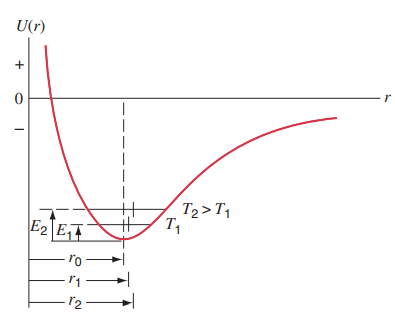
\includegraphics[width=0.4\linewidth]{images/17.molecular_potential_energy_curve.png}
	\caption{Potential energy vs separation curve}
	\label{fig:curve}
\end{figure}
\subsubsection{Microscopic Basis of Thermal Expansion}
As shown in the diagram, there is an asymmetry in the potential energy function. For distances less than equilibrium, PE increases rapidly due to strong repulsive forces. However, for distances greater than equilibrium, weaker attractive forces take over, causing PE to rise more slowly. 
\begin{enumerate}
\item At some vibrational energy, the separation $r$ goes from maximum to minimum. The asymmetry, however, keeps average separation greater than the equilibrium separation. 
\item At larger separations, the kinetic energy is lower, which causes it to contribute more to the time average.
\end{enumerate}
Since vibrational energy increases with temperature, so does average separation.
\subsection{Newton's Law of Cooling}
If the temperature difference between an object and its surroundings ($\Delta T = T_{obj} - T_{sur}$) is not too great, the rate of cooling or warming is approximately proportional to their temperature difference: 
\[ \frac{d\Delta T}{dt} = -A(\Delta T) \]
where $A$ is a constant. The negative appears because the object will always "try" to decrease the temperature difference. This is known as \textit{Newton's law of cooling}. \bigskip

If at time $t=0$ the temperature difference is $\Delta T_0$, it is 
\[ \Delta T = \Delta T_0 e^{-At} \]
some time later.
\subsection{Ideal Gases}
The results of the Constant-Volume Gas Thermometer suggests that at low enough densities, their properties converge. This gives us the concept of an \textit{ideal gas}, which exists at low pressures and high temperatures. Three experimental results have been observed: 
\begin{enumerate}
\item \textit{Boyle's Law}: PV = constant
\item \textit{Charles' Law}: V/T = constant
\item \textit{Gay Lussac's Law}: P/T = constant
\item \textit{Avogadro's Law}: V/n = constant
\end{enumerate}
where $n$ is the number of moles. Together, they make up the this following relation: 
\[ pV = NkT \]
where $N=nN_A$ is the number of molecules and $k = 1.38 \times 10^{-23} \; \textrm{J/K} $ is the Boltzmann Constant, and $N_A = 6.022 \times 10^{23}$ mol/molecule is Avogadro's constant. 
\[ pV = nRT \]
where $n$ is the number of moles and $R = 8.31 \; \textrm{J/mol} \cdot \textrm{K}$ is the molar gas constant. 
\end{document}